\documentclass{article}
\usepackage{polski} %moze wymagac dokonfigurowania latexa, ale jest lepszy niż standardowy babel'owy [polish] 
\usepackage[utf8]{inputenc} 
\usepackage{amsmath}
\usepackage{float}
\usepackage[OT4]{fontenc} 
\usepackage{enumitem}
\usepackage{graphicx,color} %include pdf's (and png's for raster graphics... avoid raster graphics!) 
\usepackage{url} 
\usepackage[pdftex,hyperfootnotes=false,pdfborder={0 0 0}]{hyperref} %za wszystkimi pakietami; pdfborder nie wszedzie tak samo zaimplementowane bo specyfikacja nieprecyzyjna; pod miktex'em po prostu nie widac wtedy ramek

\usepackage{float}
\usepackage{booktabs}

% Zmiana rozmiarów strony tekstu
\addtolength{\voffset}{-1cm}
\addtolength{\hoffset}{-1cm}
\addtolength{\textwidth}{2cm}
\addtolength{\textheight}{2cm}

%bardziej zyciowe parametry sterujace rozmieszczeniem rysunkow
\renewcommand{\topfraction}{.85}
\renewcommand{\bottomfraction}{.7}
\renewcommand{\textfraction}{.15}
\renewcommand{\floatpagefraction}{.66}
\renewcommand{\dbltopfraction}{.66}
\renewcommand{\dblfloatpagefraction}{.66}
\setcounter{topnumber}{9}
\setcounter{bottomnumber}{9}
\setcounter{totalnumber}{20}
\setcounter{dbltopnumber}{9}

% własny bullet list z malymi odstepami
\newenvironment{tightlist}{
\begin{itemize}
  \setlength{\itemsep}{1pt}
  \setlength{\parskip}{0pt}
  \setlength{\parsep}{0pt}}
{\end{itemize}}

%obrazkow szukamy w nastepujacym katalogu:
\graphicspath{{pics/}}



%\title{Sprawozdanie z laboratorium:\\Metaheurystyki i Obliczenia Inspirowane Biologicznie}
%\author{}
%\date{}

\begin{document}

\thispagestyle{empty} %bez numeru strony

\begin{center}
{\large{Sprawozdanie z laboratorium:\\
Implementacja local search}}

\vspace{3ex}
{\footnotesize\today}

\end{center}


\vspace{10ex}

Prowadzący: dr hab.~inż. Maciej Komosiński

\vspace{5ex}

Autorzy:
\begin{tabular}{lllr}
\textbf{Bartosz Nawrotek} & inf127297 & ISWD & bartosz.nawrotek@student.put.poznan.pl \\
\textbf{Wojciech Blachowski} & inf127259 & ISWD & wojciech.blachowski@student.put.poznan.pl
\end{tabular}

\vspace{5ex}

Zajęcia środowe, 15:10.

\vspace{35ex}

\noindent Oświadczam, że niniejsze sprawozdanie zostało przygotowane wyłącznie przez powyższych autorów,
a wszystkie elementy pochodzące z innych źródeł zostały odpowiednio zaznaczone i~są cytowane w bibliografii.  

\newpage


\section{Opis problemu}
\subsection{QAP}
Analizowany w tym sprawozdaniu problem nosi nazwę QAP (ang. \textit{Quadratic Assignment Problem}). Zdefiniowana jest w nim określona liczba obiektów oraz taka sama liczba lokalizacji. Pomiędzy obiektami określone są przepływy (np. dóbr, usług itp.), natomiast dla lokalizacji podane są odległości między nimi (nie muszą one być symetryczne - droga w jedną stronę może być krótsza). Celem jest taki przydział obiektów do lokalizacji, aby zminimalizować sumaryczny iloczyn przepływu dóbr oraz dystansu dla każdej pary obiektów. Intuicyjnie oznacza to, że obiekty, pomiędzy którymi dochodzi do dużego przepływu należy umieścić maksymalnie blisko siebie.
\par Problem posiada wiele możliwych zastosowań, przykładowo rozmieszczenie fabryk wśród wielu potencjalnych lokalizacji lub komponentów na układzie scalonym. 
\par QAP należy do problemów NP-trudnych. Algorytm dokładny sprawdzający wszystkie możliwe rozwiązania posiada złożoność czasową $O(n!)$, gdzie $n$ to liczba obiektów do rozmieszczenia.
\subsection{Wybrane instancje}
Do analizy wybrano 8 instancji pochodzących ze zbioru QAPLIB (ang. \textit{Quadratic Assignment Problem Library}). Dla najmniejszej z instancji liczba obiektów wynosi 12, natomiast dla największej 256. Pozostałe instancje posiadają wartości pośrednie. Taki wybór pozwoli odkryć potencjalne zależności pomiędzy rozmiarem instancji a wynikami zwracanymi przez poszczególne algorytmy.
\par Nazwy wybranych instancji to: \textit{chr12a, lipa30a, lipa40b, tai64c, sko81, sko100a, tho150, tai256c}.
\subsection{Implementacja}
Program znajdujący rozwiązania problemu został napisany w języku C++. Kod źródłowy składa się z dwóch klas: ,,Problem'', która reprezentuje daną instancję oraz ,,Solution'', która zawiera algorytmy szukające rozwiązania. Pliki źródłowe ważą sumarycznie około 10KB. 
\subsubsection{Algorytm losowy}
W ramach badań opracowano dwa algorytmy losowe. Ich wspólną cechą jest zamiana miejscami obiektów w rozwiązaniu w sposób przypadkowy oraz zapamiętywanie najlepszego napotkanego wyniku. Działają one tak długo, aż nie przekroczony zostanie zadany limit czasu.
\begin{itemize}
    \item Naiwna wersja algorytmu losowego
    
    Pierwszy z algorytmów dokonuje w każdej iteracji $n$ zamian parami elementów rozwiązania. Następnie liczona jest wartość funkcji celu dla nowej permutacji i jeżeli jest ona zapamiętywana jeśli jest lepsza od ostatniej napotkanej.
    \item Ulepszona wersja algorytmu losowego
    
    W ulepszonej wersji algorytmu losowego po każdorazowej zmianie miejscami pary elementów rozwiązania dokonywane jest wyznaczanie nowej wartości funkcji celu. Obliczenia dokonywane są poprzez naniesienie ,,poprawki'' na wartość sprzed zamiany. W ten sposób liczenie wartości funkcji celu bierze pod uwagę jedynie wpływ dokonanej zmiany i odbywa się ze złożonością O(n). Algorytm dzięki temu może w tym samym czasie dokonać znacznie większej eksploracji możliwych rozwiązań niż jego naiwna wersja.
\end{itemize}
\subsubsection{Prosta heurystyka}
Algorytm heurystyczny działa poprzez przypisanie konkretnego obiektu do losowo wybranej lokalizacji, a następnie przypisanie pozostałych obiektów do każdego następnego miejsca w sposób zachłanny. Spośród wszystkich nieprzypisanych obiektów wybierany jest ten, dla którego funkcja celu wzrośnie jak najmniej.
\par Algorytm wykonywany jest wielokrotnie w zadanym czasie, każdorazowo losując początkową lokalizację.
\section{Opis użytych operatorów sąsiedztwa}
Wykorzystany operator sąsiedztwa zamienia miejscami dwa obiekty w rozwiązaniu. Rozmiar sąsiedztwa jest więc równy liczbie wszystkich możliwych par obiektów i wynosi $n(n-1)/2$, gdzie $n$ to liczba obiektów.
\section{Porównanie działania algorytmów}
Porównano działanie 5 algorytmów na wszystkich 8 analizowanych instancjach problemu. Dla uproszczenia zapisu przyjęto następujące oznaczenia algorytmów:
\begin{itemize}
    \item Greedy Local Search: GLS,
    \item Steepest Local Search: SLS,
    \item Prosta heurystyka: H,
    \item Naiwna wersja algorytmu losowego: NRS,
    \item Ulepszona wersja algorytmu losowego: LNRS.
\end{itemize}
W celu uzyskania miarodajnych pomiarów, każdy algorytm został uruchomiony dziesięciokrotnie dla każdej z instancji. 
\subsection{Jakość rozwiązania}
Pierwszą miarą porównawczą algorytmów jest jakość rozwiązania rozumiana jako iloraz wartości funkcji celu rozwiązania optymalnego oraz wartości funkcji celu uzyskanego wyniku. Optymalna wartość jakości wynosi więc 1 a jakości rozwiązań o mniejszej wartości funkcji celu zawierają się w przedziale $ \langle 0, 1 ) $ przy założeniu nieujemnej określoności obu macierzy.
\par Uzyskane rezultaty przedstawia rysunek \ref{fig:quality_mean}. Znajdują się na nim wykresy pudełkowe pokazujące wyniki działania każdego z algorytmów. Zaskakujcym wydawać się mogą wyniki uzyskane przy pomocy algorytmu losowego LNRS, wysokie wartości jakości dla tego algorytmu mogą świadczyć o trudności analizowanych instancji i o niskiej korelacji wartości funkcji celu oraz permutacji nawet w kontekście odpowiednio dobranego operatora sąsiedztwa. Co potwierdza jego efektywność w eksploracji przestrzeni rozwiązań. Kolejny rysunek \ref{fig:quality_min} ukazuje słabą skuteczność heurystyki dla instancji \texit{chr12a, tai64c, tai256c}. O ile w przypadku instancji \textit{chr12a}, żaden z zastosowanych algorytmów nie jest szczególnie skuteczny, to dla instancji \texit{tai64c, tai256c} jej wyniki są znacząco gorsze. Może to świadczyć o podobieństwie krajobrazu funkcji celu tych instancji.
\begin{figure}[H]
	\centering
	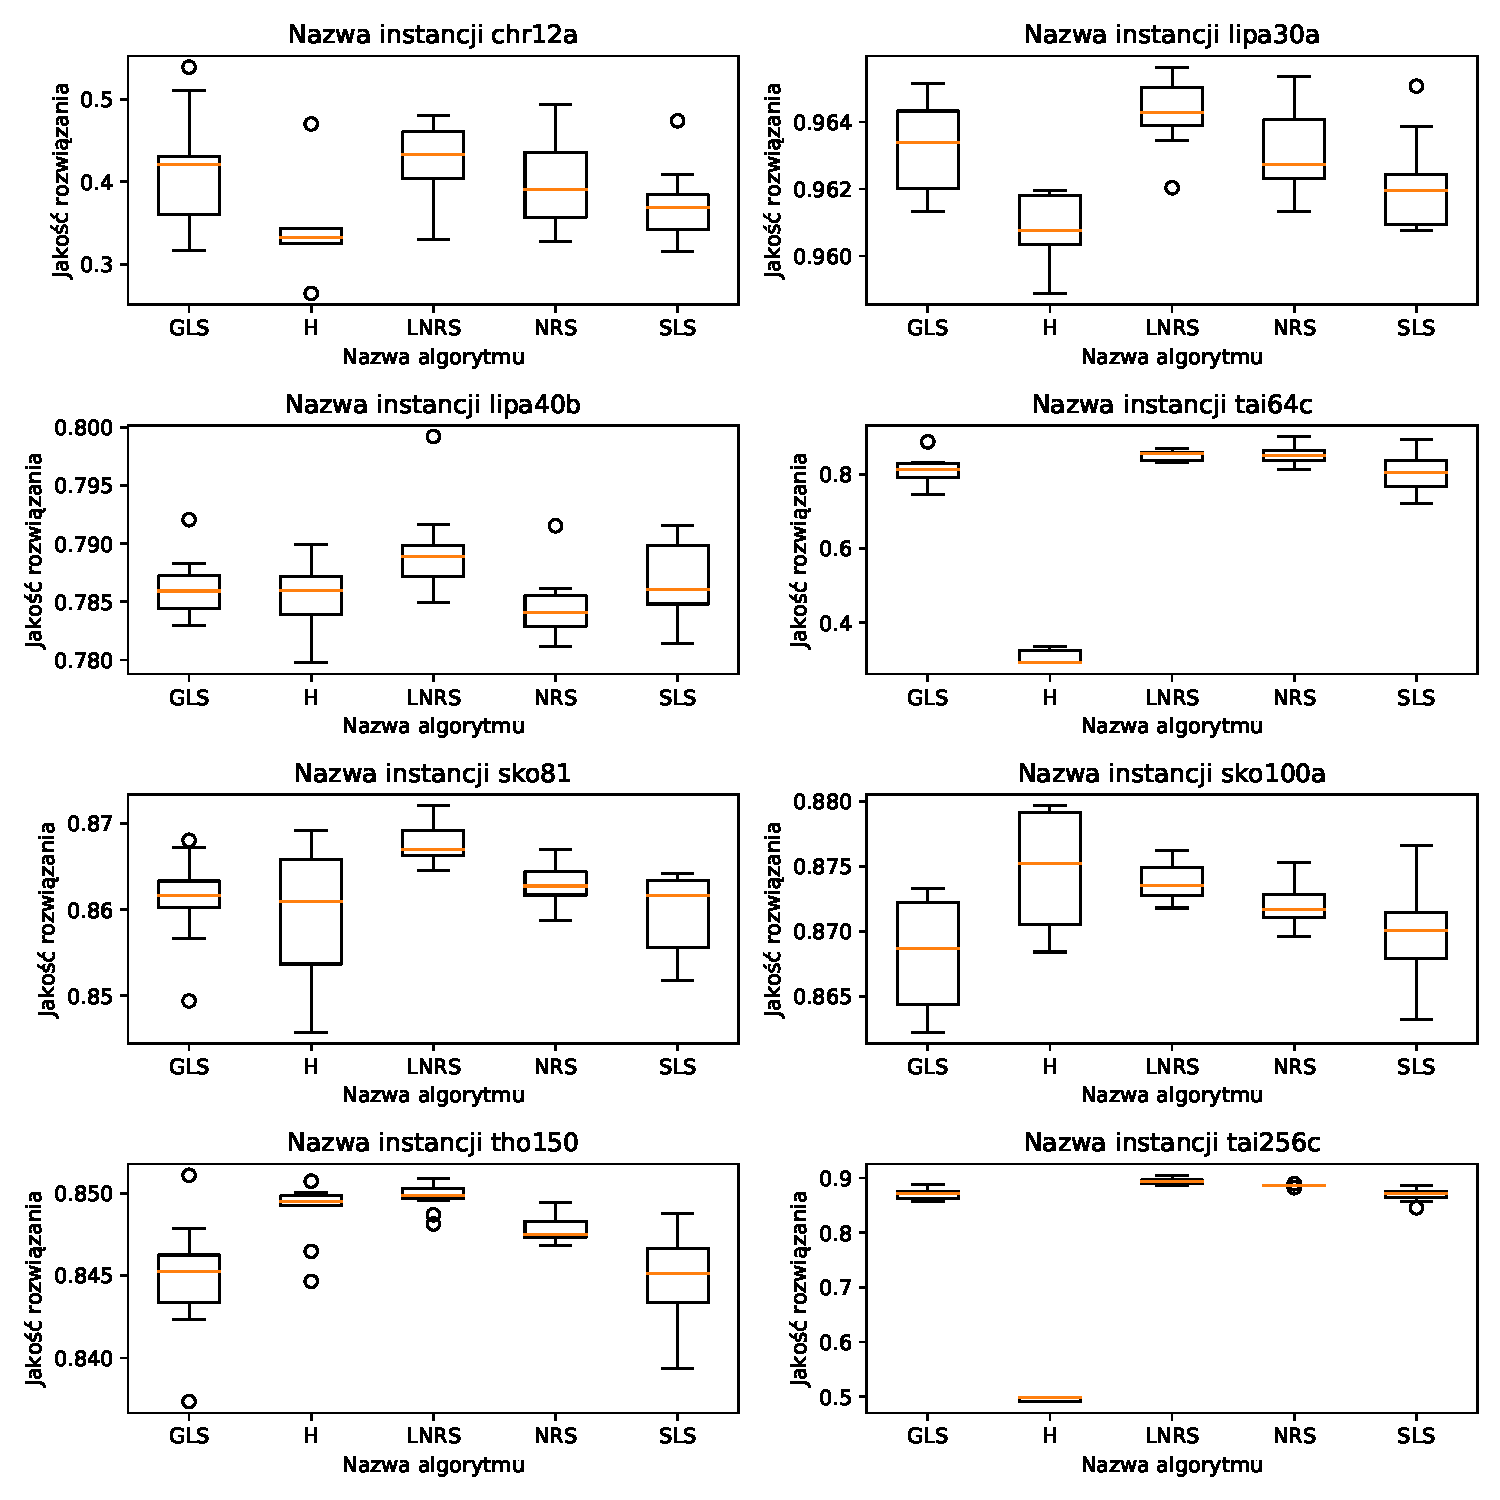
\includegraphics[width=\linewidth]{figs/quality_mean.pdf}
	\caption{Jakość rozwiązań uzyskana za pomocą analizowanych algorytmów dla poszczególnych instancji. Instancje są uporządkowane w kolejności rosnącego rozmiaru. }
	\label{fig:quality_mean}
\end{figure}

\begin{figure}[H]
	\centering
	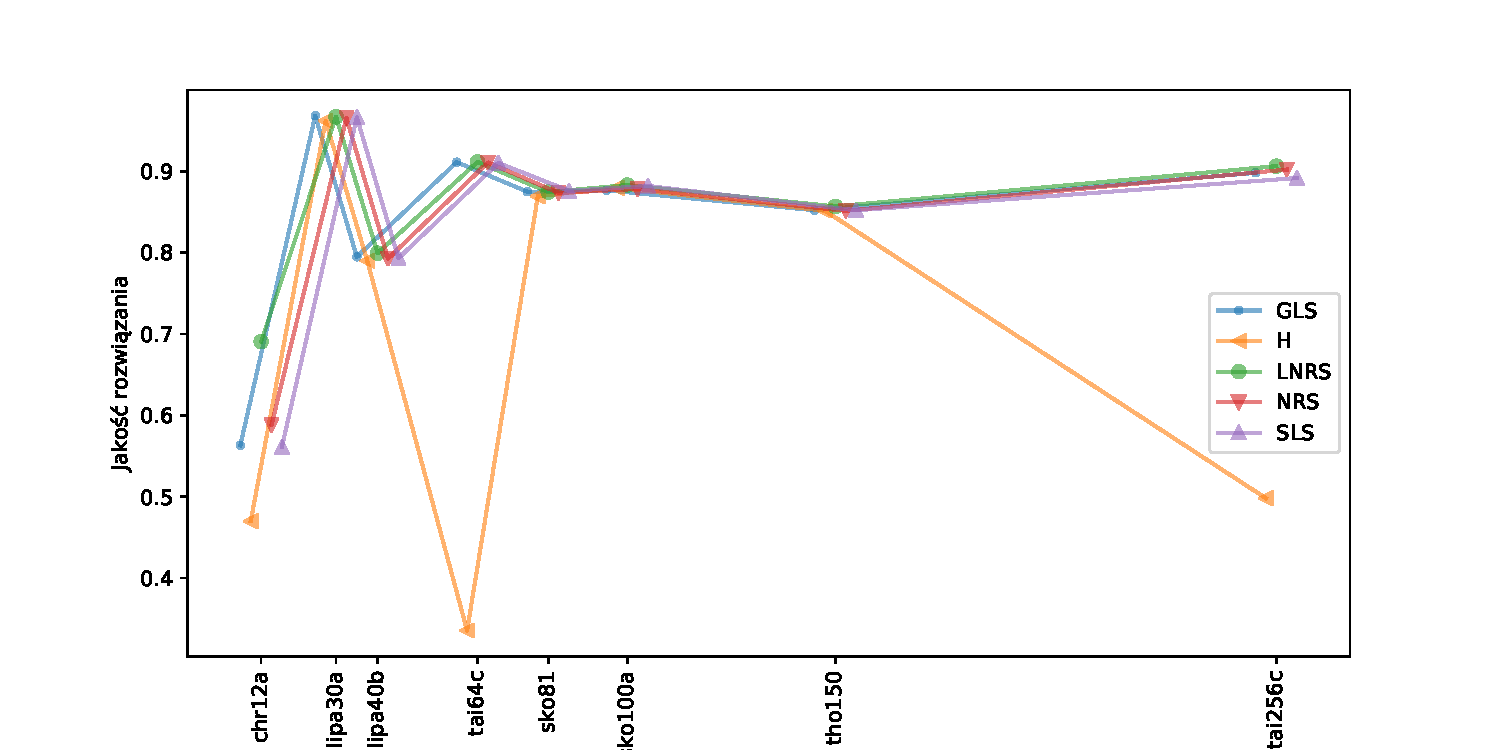
\includegraphics[width=\linewidth]{figs/quality_best.pdf}
	\caption{Jakość najlepszego rozwiązania uzyskana za pomocą analizowanych algorytmów dla poszczególnych instancji. Instancje są uporządkowane w kolejności rosnącego rozmiaru.}
	\label{fig:quality_mean}
\end{figure}
\subsection{Czas działania}
Średnie czasy wraz z z odchyleniem standardowym z 10 uruchomień algorytmów dla każdej z instancji przedstawiono na rysunku \ref{fig:time_mean}. Na podstawie wykresu można zauważyć, że długość przetwarzania rośnie wykładniczo wraz ze wzrostem rozmiaru instancji. Dla algorytmów Local Search ten wynik prawdopodobnie spowodowany jest rozmiarem sąsiedztwa, kolejnym czynnikiem mogącym mieć wpływ jest gęstość występowania lokalnych optimów w krajobrazie funkcji celu. Pozostałe algorytmy zostały uruchamiane z ograniczeniem czasu wykonywania do długości bliskiej czasowi wykonania algorytmów Local Search, co zostało potwierdzone na wykresie.
\begin{figure}[H]
	\centering
	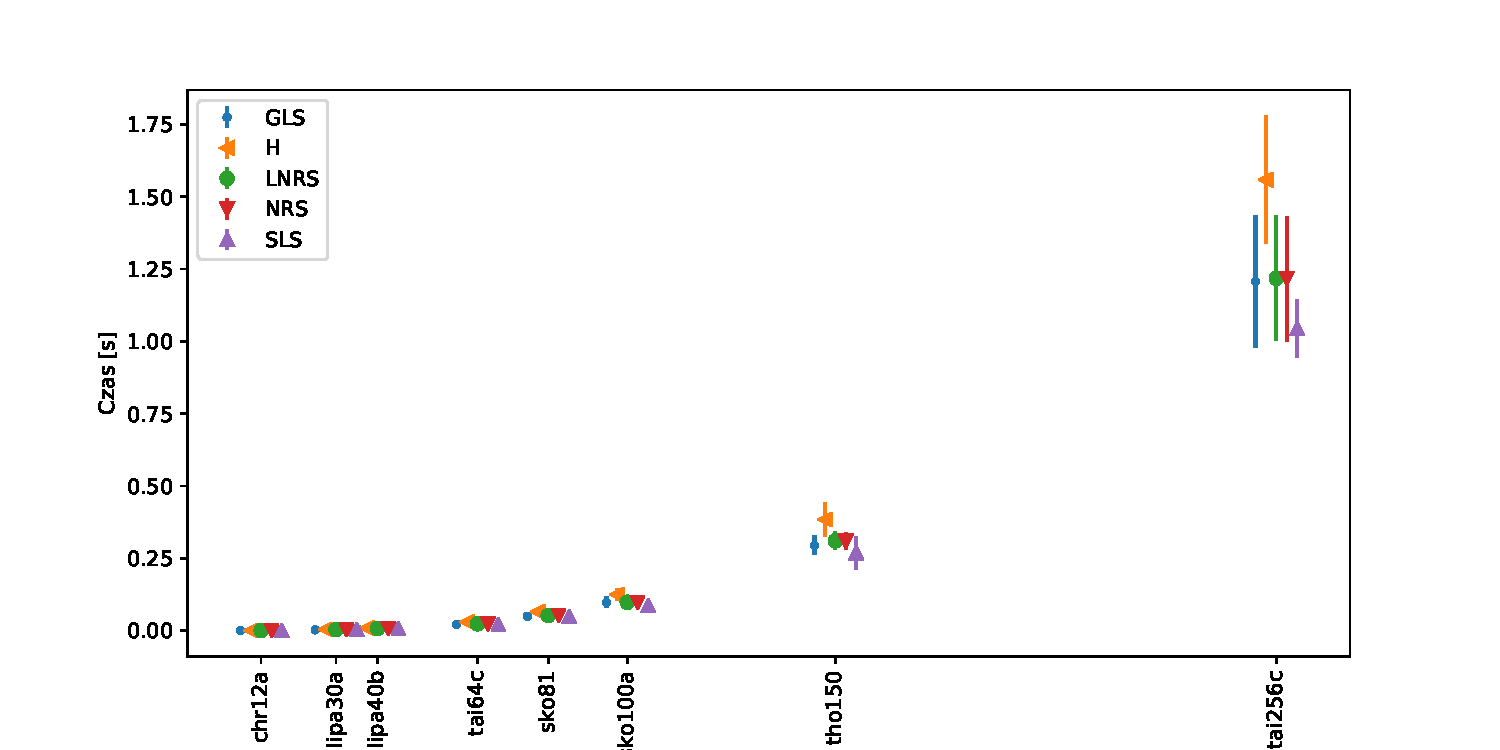
\includegraphics[width=\linewidth]{figs/mean_time.pdf}
	\caption{Czas działania algorytmów dla wybranych instancji.}
	\label{fig:time_mean}
\end{figure}

\subsection{Efektywność algorytmów}
Na rysunku \ref{fig:efficiency} przedstawiono efektywność analizowanych algorytmów. Efektywność definiujemy jako iloraz uzyskanej jakości oraz czasu przetwarzania. 
\par 
Decydująca okazuje się długość obliczeń, co można zaobserwować na przykładzie wyników dla instancji \textit{chr12a} oraz \textit{lipa30a}. Algorytmy uzyskują średnio 2 razy lepszą jakość dla instancji \texit{lipa30a} niż \textit{chr12a}. Ponieważ jednak przetwarzanie dla instancji o większym rozmiarze trwa zdecydowanie dłużej niż dla mniejszej instancji, efektywność jest lepsza dla instancji \textit{chr12a}, mimo gorszej jakości. Kolejną ważną obserwacją jest uzyskanie najwyższych wartości efektywności przez algorytmy lokalnego przeszukiwania, co było oczekiwanym wynikiem, ponieważ świadczy to o ich eksploatacji wyników początkowych.
\begin{figure}[H]
	\centering
	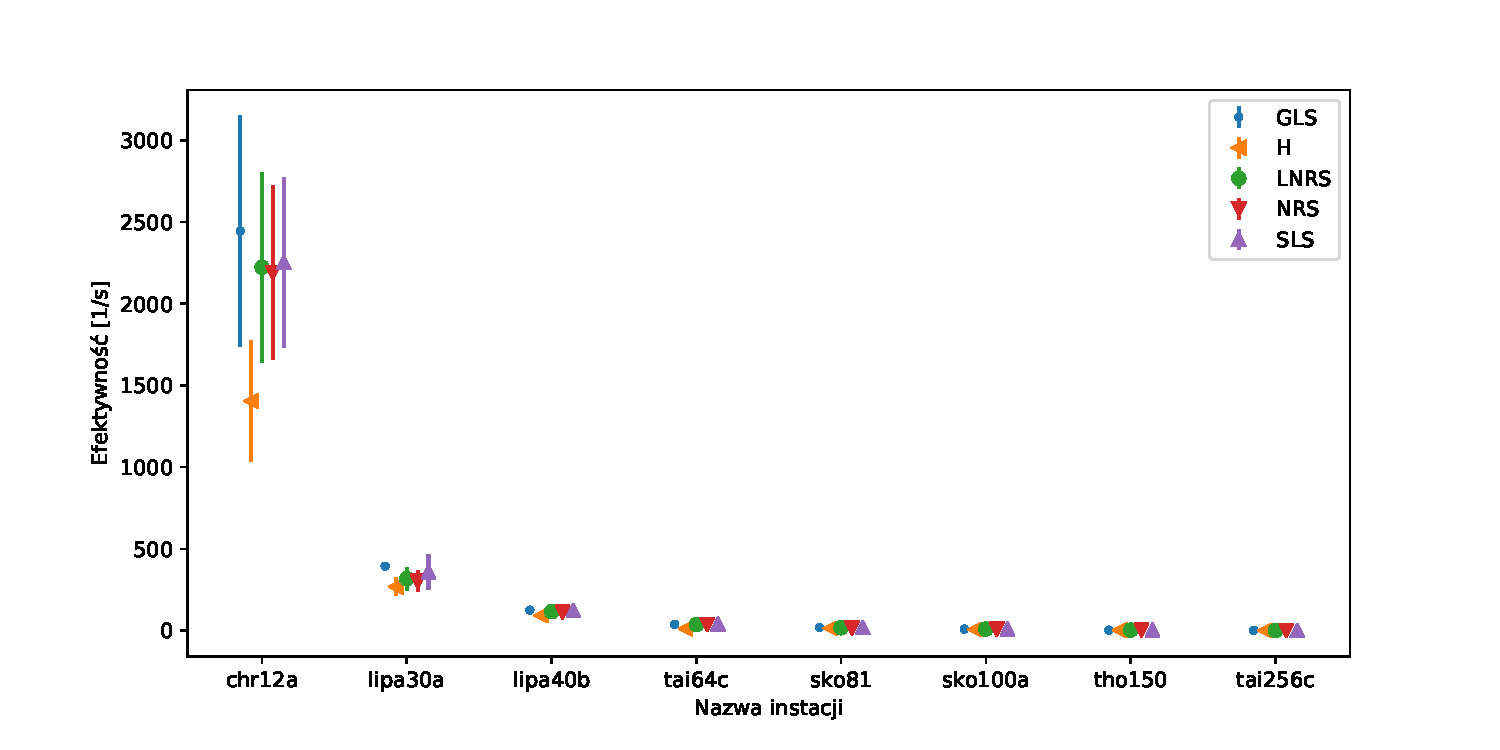
\includegraphics[width=\linewidth]{figs/efficiency.pdf}
	\caption{Efektywność algorytmów dla wybranych instancji.}
	\label{fig:efficiency}
\end{figure}

\subsection{Średnia liczba kroków algorytmu i liczba ocenionych rozwiązań dla algorytmów Local Search}
Na wysunku \ref{fig:num_obj_val_calls} przedstawiono liczbę ocenionych rozwiązań w funkcji instancji problemu. Uzyskane wyniki ukazują największą eksplorację przestrzeni rozwiązań przez algorytm LNRS, oraz wysoką eksplorację w przypadku algorytmów przeszukiwania lokalnego. Te wysokie wartości w przypadku algorytmów przeszukiwania lokalnego spowodowane są szybkim przeglądaniem sąsiedztwa lub w przypadku algorytmu LNRS wykorzystaniem permutacji pośrednich podczas generowania nowej permutacji losowej poprzy zastosowaniu mechanizmu ,,poprawek''. Algorytmy pozostałe charakteryzują się stosunkowo rzadkim ocenianiem rozwiązań, co potwierdzają uzyskane wyniki.

\begin{figure}[H]
	\centering
	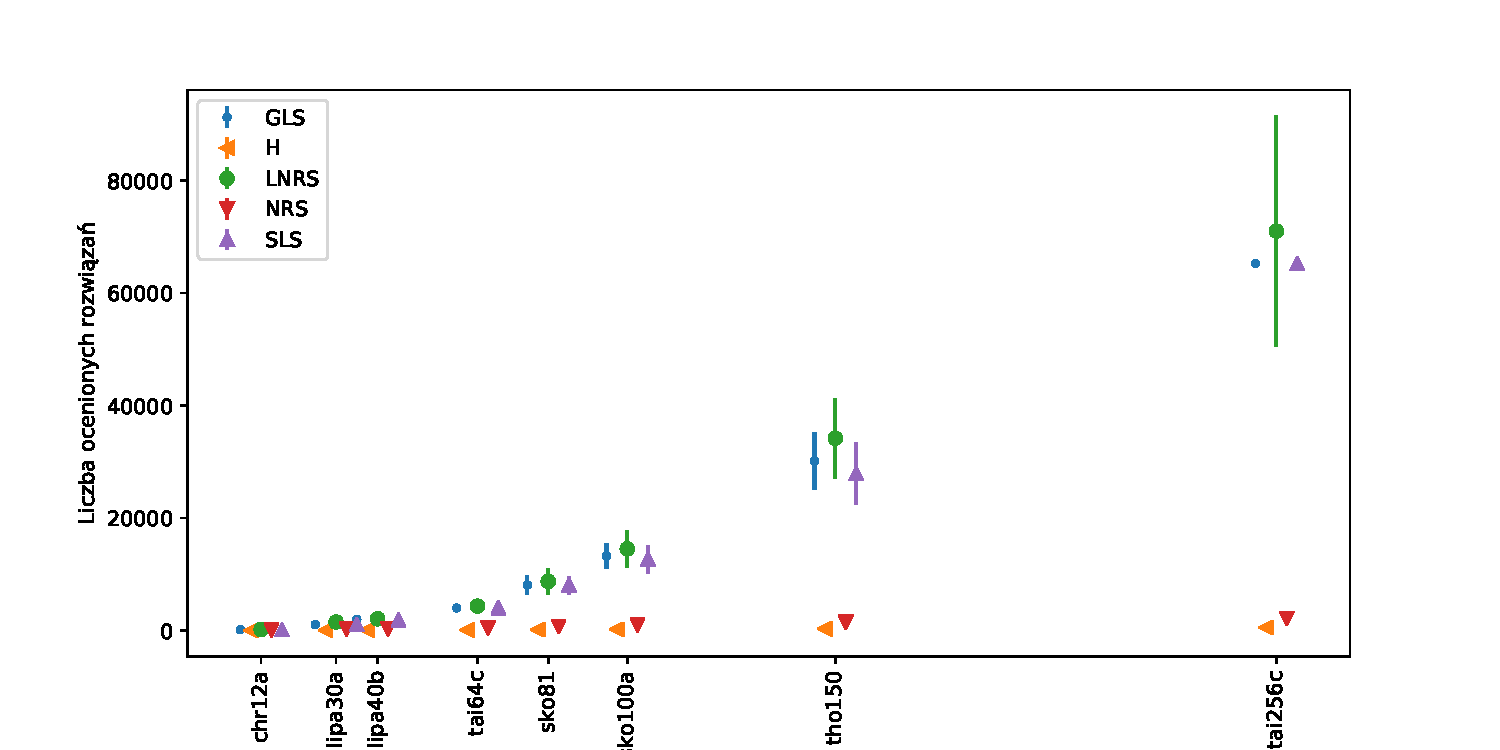
\includegraphics[width=\linewidth]{figs/num_obj_val_calls.pdf}
	\caption{Liczba ocenionych rozwiązań przez analizowane algorytmy dla poszczególnych instancji problemu.}
	\label{fig:num_obj_val_calls}
\end{figure}

\section{Jakość rozwiązania początkowego vs. jakość rozwiązania końcowego}
Na rysunku \ref{fig:quality_start_vs_quality} przedstawiono zależność jakości końcowego rozwiązania od jakości początkowego, losowanego rozwiązania dla dwóch wybranych instancji (\textit{chr12a} oraz \textit{sko100a}). Analizy dokonano dla algorytmów Greedy Local Search oraz Steepest Local Search.
\par Dla instancji \textit{sko100a} można zaobserwować wyraźną korelację liniową pomiędzy końcowym i początkowym wynikiem. Jest to najbardziej spodziewany rezultat i może wynikać z pewnej okresowości krajobrazu fukcji celu dla wybranego operatora sąsiedztwa. W przypadku instancji \textit{chr12a} zależność między zmiennymi jest znacznie mniej widoczna. Dojście do względnie wysokiej wartości (np. zbliżonej do 0.6) jest możliwe dla wielu różnych rozwiązań początkowych, zarówno o niskiej jak i wysokiej jakości, co świadczy o nieregularności krajobrazu funkcji celu dla operatora 2OPT.
\begin{figure}[H]
	\centering
	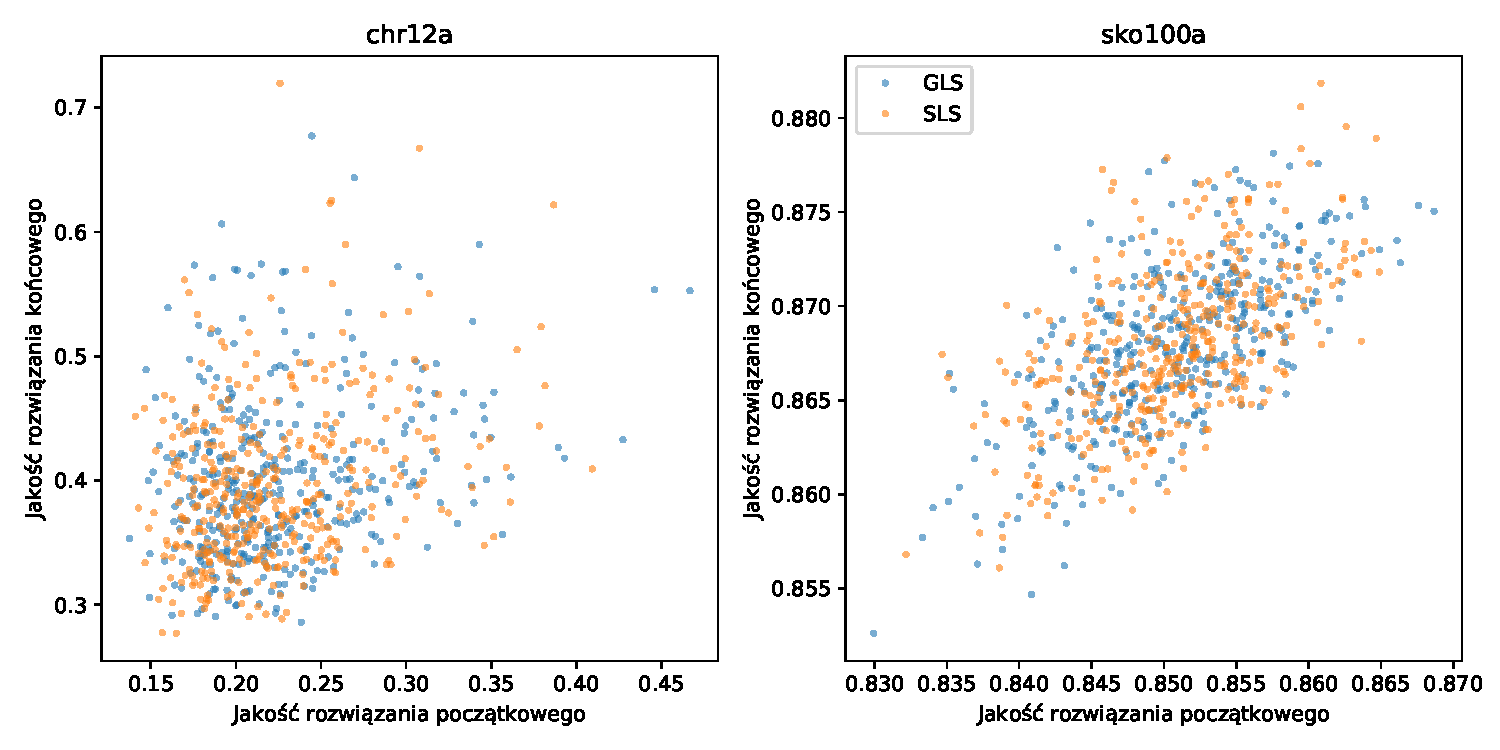
\includegraphics[width=\linewidth]{figs/quality_start_vs_quality.pdf}
	\caption{Wykres jakości ostatecznego rozwiązania w zależności od jakości rozwiązania początkowego dla instancji \textit{chr12a, sko100a}.}
	\label{fig:quality_start_vs_quality}
\end{figure}

\section{Zależność wartości funkcji celu znalezionego rozwiązania od liczby uruchomień }
Takie kształty funkcji minimalnej wartości funkcji celu w zależności od liczby restartów były oczekiwanym wynikiem. W przypadku wyników na wykresach na rysunku \ref{fig:quality_min} można zaobserwować znaczną poprawę w początkowej części wykresu oraz coraz mniejszą poprawę rozwiązania podaczas kolejnych uruchomień. Taki kształt wynika z przeszukiwania ogromnej przestrzeni rozwiązań. Ciekawym może wydawać się wykres dla instancji \textit{tai256c}, który pokazuje, że może istnieć niskie prawdopodobieństwo trafienia w punkt przestrzeni o niższej wartości funkcji celu nawet po prawie 400 restartach algorytmu. Pokazuje to zasadność wielokrotnego stosowania algorytmów lokalnego przeszukiwania. Dla każdej analizowanej instancji lepsze wyniki uzyskano w przypadku wykorzystania algorytmu SLS, co w ogólności nie musi być prawdą.
\begin{figure}[H]
	\centering
	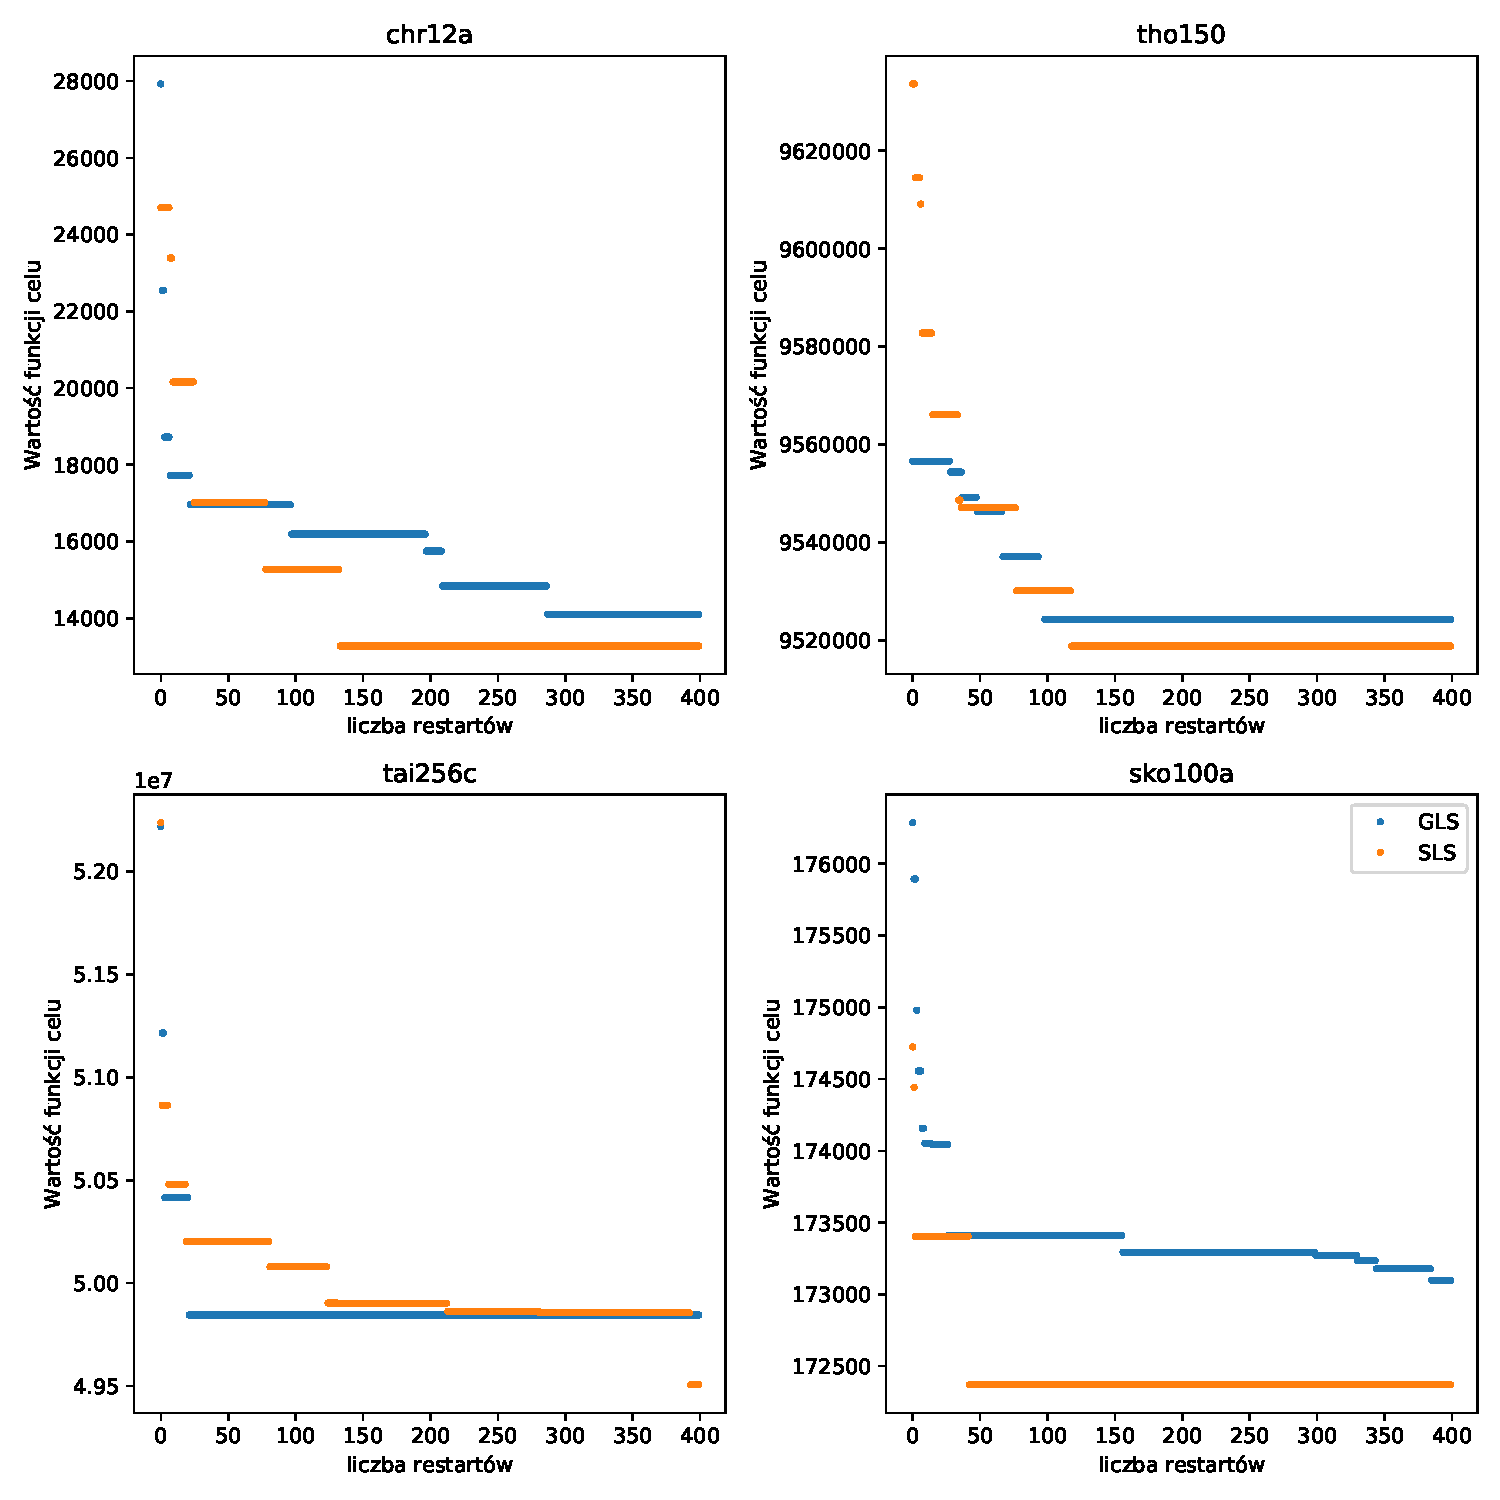
\includegraphics[width=\linewidth]{figs/min_acc_end_obj_val.pdf}
	\caption{Wykres minimalnej wartości funkcji celu w zależności od liczby uruchomień algorytmów w trybie multi-random start dla instancji \textit{chr12a, tho150, tai256, sko100a}.}
	\label{fig:quality_min}
\end{figure}

Dla wyników na rysunku \ref{fig:quality_mean} uzyskane kształty wynikają z dążenia kumulatywnej wartości średniej z uzyskanych wartości funkcji celu do stałej wartości. Taki wynik charakteryzuje algorytmy przeszukiwania nie wykorzystujące informacji o poprzdnich wywołaniach i świadczy to o braku gwarancji uzyskanie rozwiązania co najmniej tak dobrego jak w poprzednim wywołaniu. Ten test jest przykładem aplikacji mocnego prawa wielkich liczb Kołomogorowa w optymalizacji, którego założenia o niezależności zmiennych losowych o tym samym rozkładzie oraz o ograniczonej wartości średniej (uzyskanych wyników) są spełnione.

\begin{figure}[H]
	\centering
	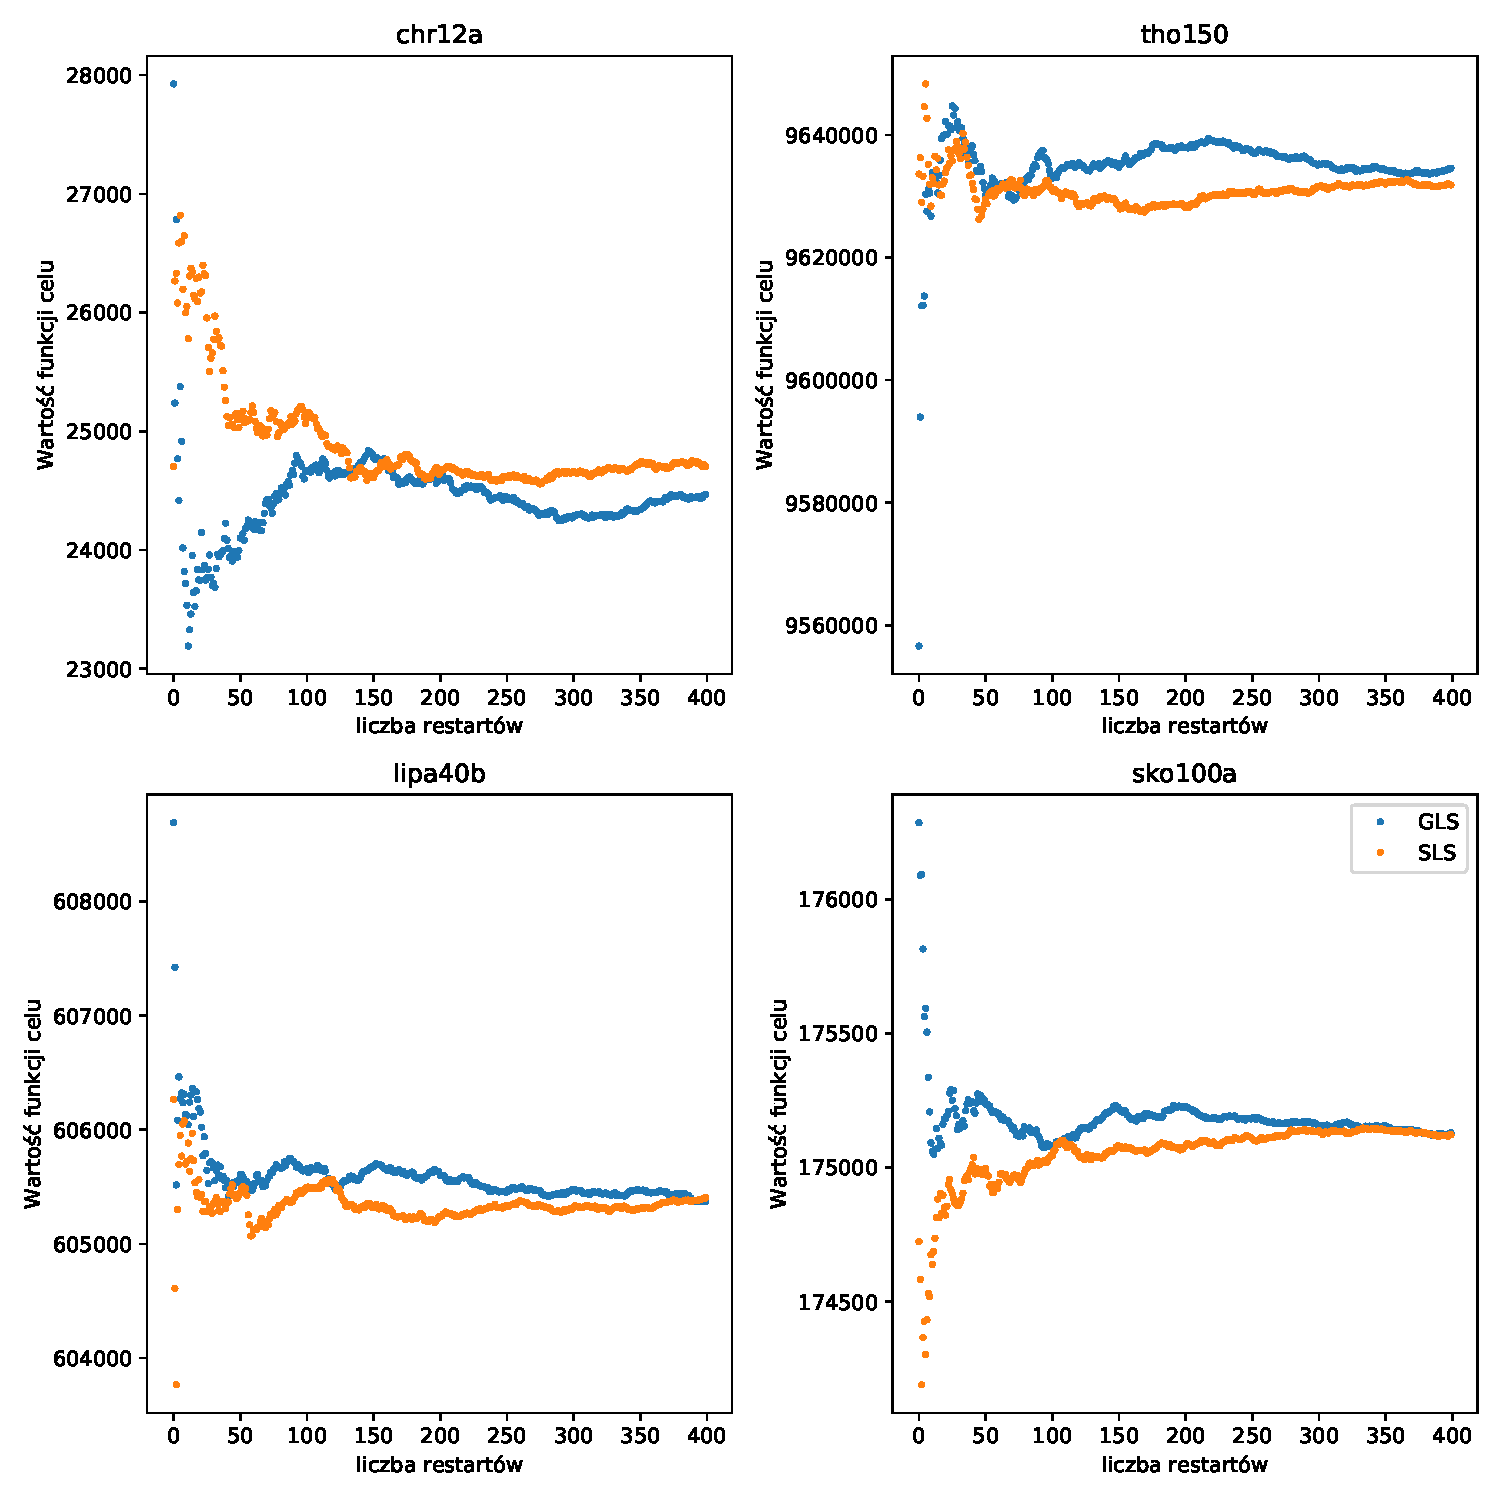
\includegraphics[width=\linewidth]{figs/mean_acc_end_obj_val.pdf}
	\caption{Wykres średniej wartości funkcji celu w zależności od liczby uruchomień algorytmów w trybie multi start dla instancji \textit{chr12a, tho150, lipa40b, sko100a}.}
	\label{fig:quality_mean}
\end{figure}

\section{Podobieństwo znajdowanych rozwiązań lokalnie optymalnych dla dwóch wybranych instancji}
Podobieństwo dwóch rozwiązań definiujemy jako liczbę miejsc w obu permutacjach, które posiadają taką samą wartość. Dla interpretacji QAP jako problemu przydziału obiektów do danych lokalizacji oznacza to, że rozwiązania są tym bardziej podobne, im więcej obiektów zostało przypisanych do tych samych lokalizacji w obu rozwiązaniach.

Wynikiem oczekiwanym było zaobserwowanie korelacji podobieństwa wraz z jakością rozwiązania. Niestety zdefiniowana miara podobieństwa nie pozwoliła na zaobserwowanie tego zjawiska, ze względu na bardzo rzadkie dopasowanie poszczególnych elementów w permutacji. Na rysunku \ref{fig:similarity_opt} pokazano, że nawet dla najmniejszego z wybranych rozmiarów instancji istnieje bardzo mało rozwiązań podobnych do rozwiązania optymalnego na choć 4 z 12 elementów tej permutacji. Trudność w odszukaniu podobieństwa między instancjami o większym rozmiarze jest jeszcze większa, co ukazano na wykresie dla instancji \texit{tai256c}.
\begin{figure}[H]
	\centering
	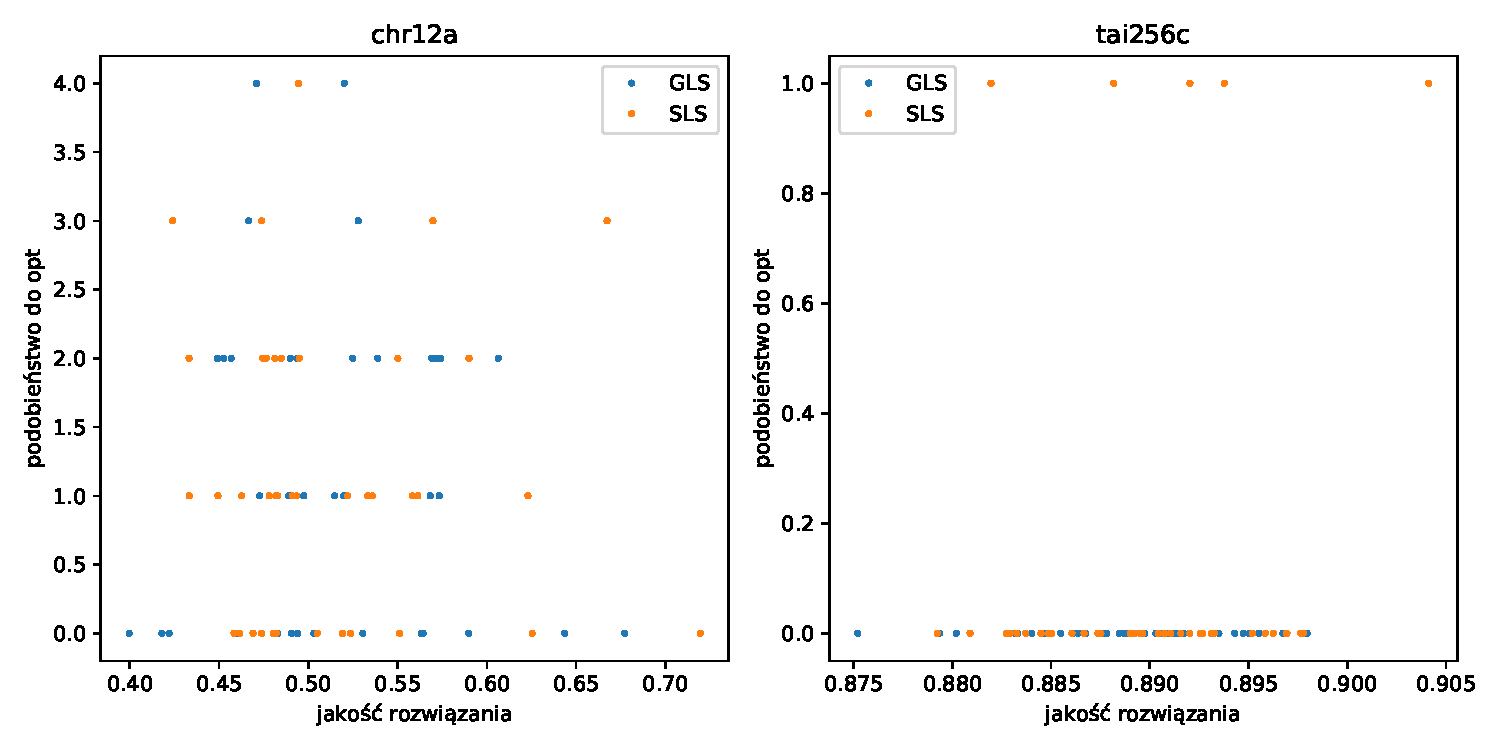
\includegraphics[width=\linewidth]{figs/quality_best_numit_vs_similarity_opt.pdf}
	\caption{Wykresy przedstawiają wartości miary podobieństwa rozwiązań do rozwiązania optymalnego dla instancji \textit{chr12a, tai256c}.}
	\label{fig:similarity_opt}
\end{figure}

Na kolejnym rysunku \ref{fig:similarity_interior} ukazano wartość miary podobieństwa pary uzyskanych permutacji w funkcji różnic ich jakości. Wykresy pokazują, że im dwa rozwiązania są bardziej do siebie podobne, tym mniejsza jest ich różniżnica jakości. Taka obserwacja może świadczyć o korelacji jakości ze zdefiniowaną miarą podobieństwa, co jest oczekiwanym wynikiem, którego niestety nie udało się uzyskać w porównaniu z rozwiązaniem optymalnym. Wykres dla instancji \textit{tai256c} posiada trochę inną charakterystykę dla wartości miary podobieństwa równej 0, co może wskazywać, że lokalne optima często mają tę samą wartość na jednej z pozycji permutacji.

\begin{figure}[H]
	\centering
	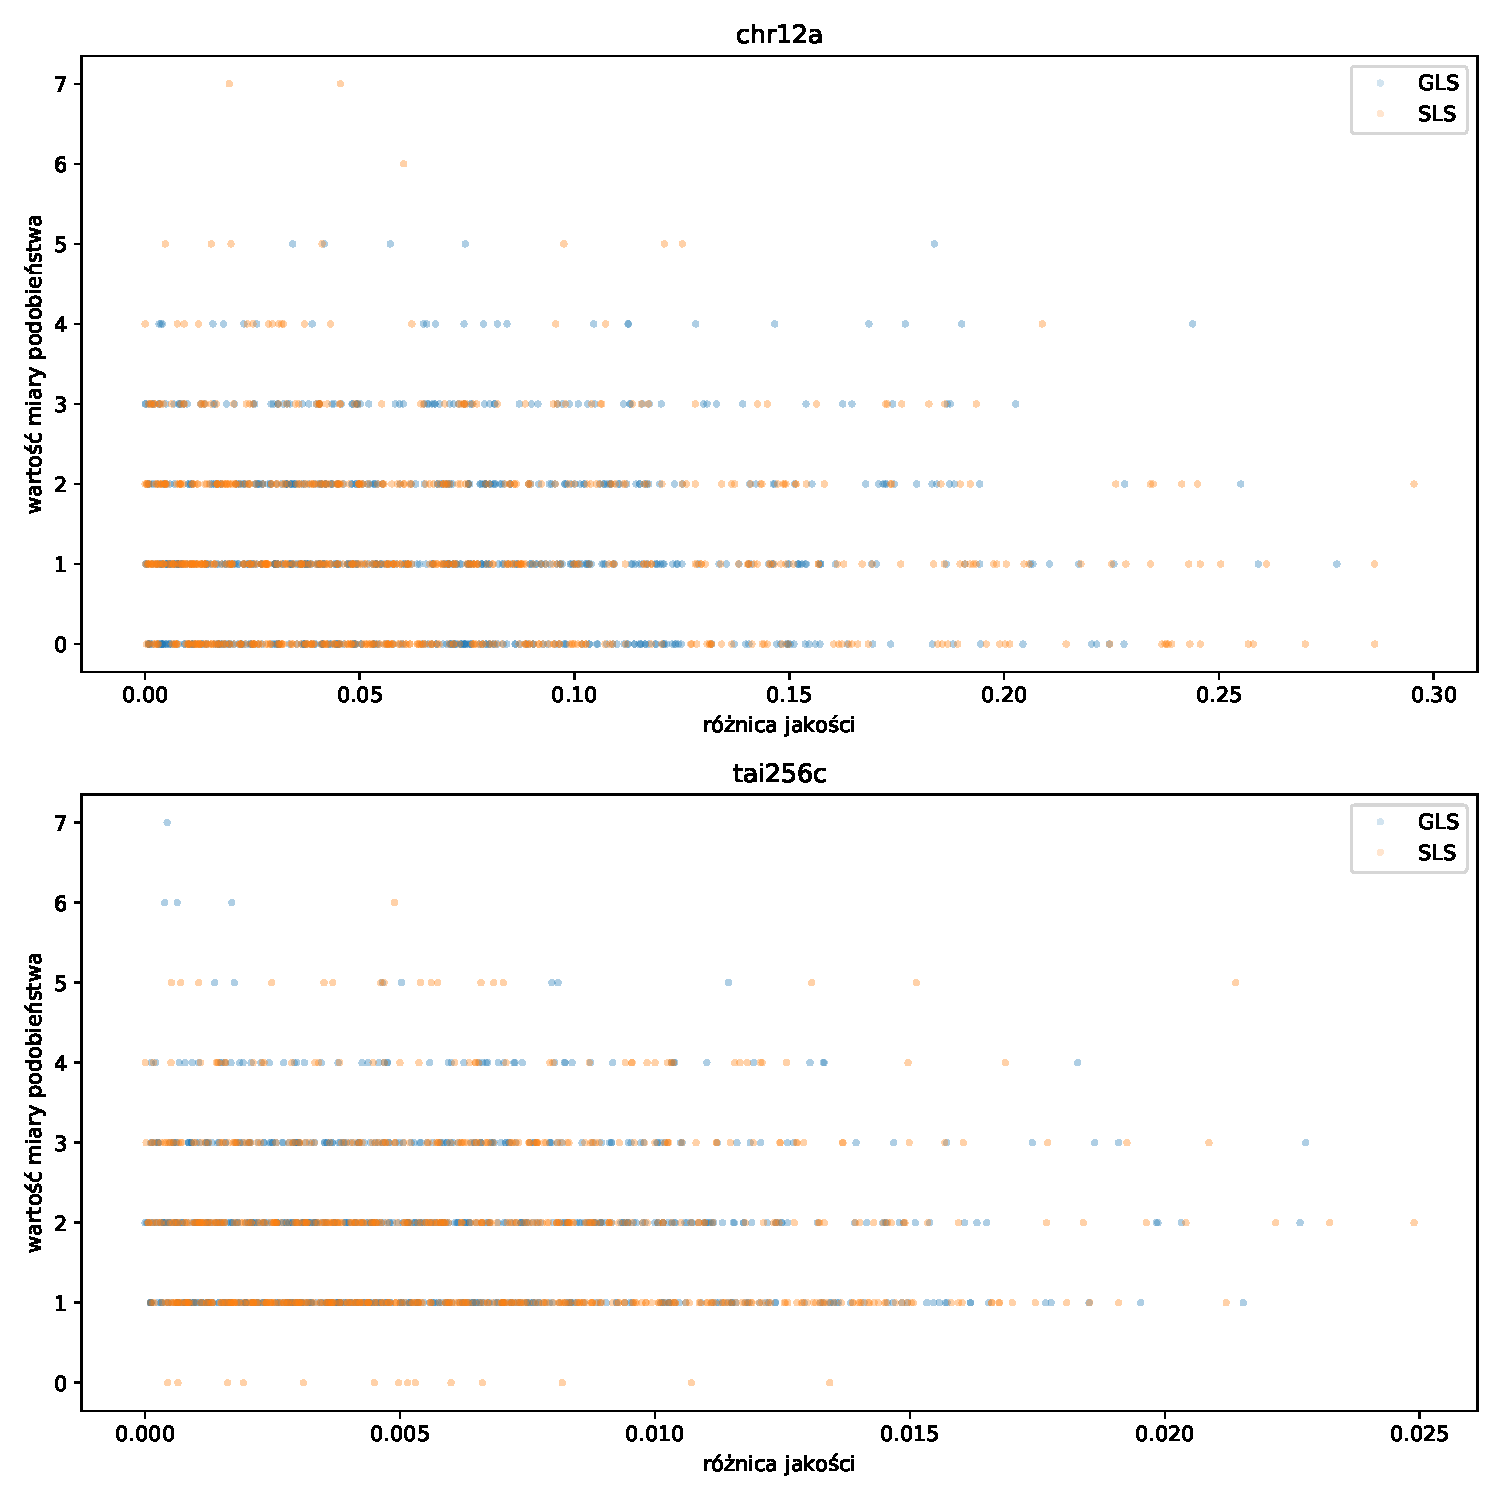
\includegraphics[width=\linewidth]{figs/delta_quality_interior_vs_similarity.pdf}
	\caption{Wykres średniej wartości funkcji celu w zależności od liczby uruchomień algorytmów w trybie multi start dla instancji \textit{chr12a, tho150, lipa40b, sko100a}.}
	\label{fig:similarity_interior}
\end{figure}

\section{Wnioski}
Jednym z najbardziej zaskakujących wniosków z dokonanej analizy jest skuteczność algorytmów losowych dla wybranych instancji problemu. Oraz wysoka skuteczność prostej heurystyki dla większości analizowanych instancji problemu. Algorytmy te, w szczególności ulepszona wersja algorytmu losowego, uzyskują niejednokrotnie rozwiązania o lepszej jakości niż algorytmy Greedy i Steepest Local Search. Ich ogromnym atutem jest efektywność w eksploracji przestrzeni. Kolejnym wnioskiem, jaki udało się wykazać jest trudność optymalizacji instancji \textit{chr12a}, co było zauważalne zarówno na wykresach uzyskiwanej jakości rozwiązań średnich/najlepszych, jak i na wykresie jakości ostatecznego rozwiązania w zależności od jakości początkowego rozwiązania, które wskazywało na wysoką nieregularność krajobrazu. Kolejnym ciekawym wnioskiem jest ukazana charakterystyka instancji \textit{tai256c}. Z jednej strony prawie wszystkie wywołania algorytmów lokalnego przeszukiwania mają tę samą wartość na jednej z pozycji, a z drugiej strony rozwiązanie optymalne wydaje się na tej pozycji różnić, na co wskazuje rysunek \ref{fig:similarity_opt}.
\par 
\section{Trudności jakie napotkano}
Niestety nie udało się pokazać sensownej zależności między podobieństwem do rozwiązania optymalnego a jakością uzyskanego rozwiązania. Prawdopodobnie dla problemu QAP trudno jest zdefiniować lepszą miarę podobieństwa.

\section{Propozycje udoskonaleń}
Jednym z pomysłów jest próba połączenia zalet algorytmów lokalnego przeszukiwania oraz algorymu LNRS. Polegała by ona na generowaniu instancji dla kolejnego wywołania algorytmu na podstawie już istniejącego optimum lokalnego. Byłoby ono wykorzystane do wygenerowania nowej instancji losowej, podczas tego generowania byłyby oceniane permutacje pośrednie z wykorzystaniem funkcji nanoszenia ,,poprawek''.

Kolejnym możliwym udoskonaleniem działania algorytmów lokalnego przeszukiwania byłoby zastosowania innego operatora sąsiedztwa, którym mogłoby być sąsiedztwo 3OPT powiększone o 2OPT.

Można również rozważyć wykorzystanie heurystyki do generowania początkowych rozwiązań dla algorytmów przeszukiwania lokalnego.

\end{document}
